\part{Other Post Processing Techniques}
\frame{\partpage}

  \begin{frame}
	\frametitle{Colour Correction}
	\begin{columns}
		\begin{column}{0.5\textwidth}
			\begin{itemize}
				\item Process of taking an image, convert each colour in the image to a some other colour
				\item Mimic a specific film stock, provide coherent look or provide a mood
			\end{itemize}
		\end{column}
		\begin{column}{0.5\textwidth}
			\begin{center}
				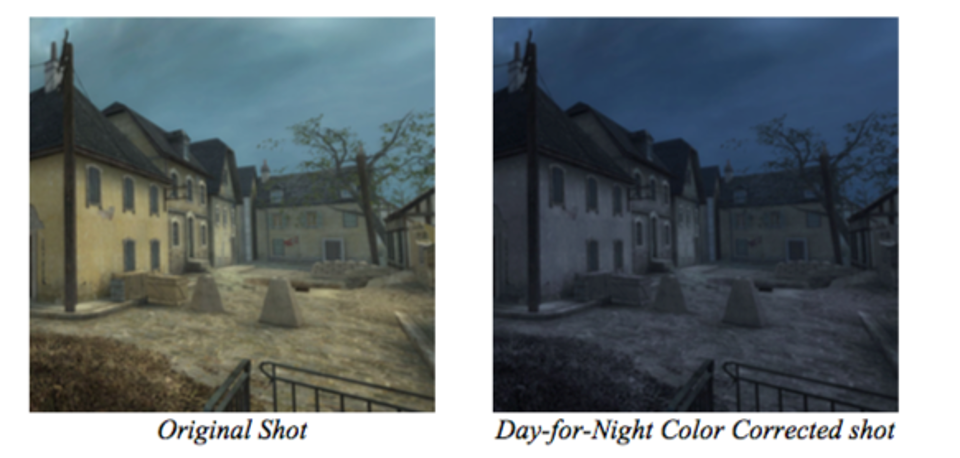
\includegraphics[width=\textwidth]{colour_correction_daynight}
			\end{center}
		\end{column}
	\end{columns}
\end{frame}


\begin{frame}
	\frametitle{Colour Correction Again}
		\begin{columns}
		\begin{column}{0.5\textwidth}
			\begin{itemize}
				\item Depending on the technique this could involve manipulating the colours using a Filter Kernel
				\item Or we could use a colour palette (see Colour Grading) 
			\end{itemize}
		\end{column}
		\begin{column}{0.5\textwidth} 
			\begin{center}
				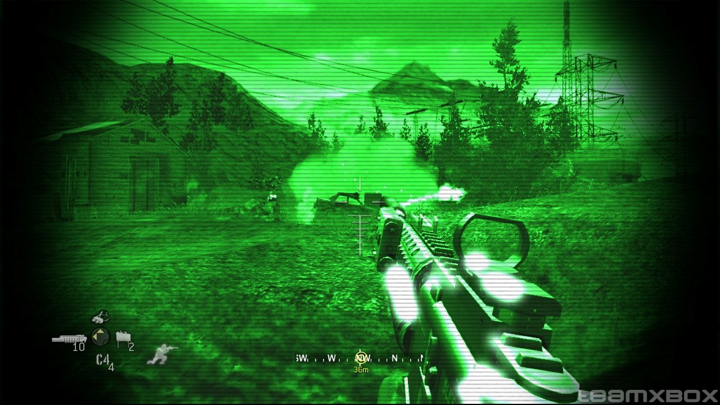
\includegraphics[width=\textwidth]{colour_correction_nightvision}
			\end{center}
		\end{column}
	\end{columns}
\end{frame}

\begin{frame}{Blur}
	\begin{itemize}
		\item\pause This often used as a basis for other techniques such as Depth of Field
		\item\pause To achieve blurring we apply a filter to the texture lookup of the texture render target
		\item\pause We can apply many different filters, one of the simplest is a Box Filter
		\item\pause With a box filter we sample 4 points around the point we are interested in and take an average
	\end{itemize}
\end{frame}

\begin{frame}
	\frametitle{Motion Blur}
\begin{columns}
	\begin{column}{0.5\textwidth}
		\begin{itemize}
			\item If an object moves very fast through you Field of view it can appear that the object leaves a slight ghost of itself
			\item There are several ways of implementing this, we can use the actual speed of the object to determine the amount of blur
		\end{itemize}
	\end{column}
	\begin{column}{0.5\textwidth} 
		\begin{center}
			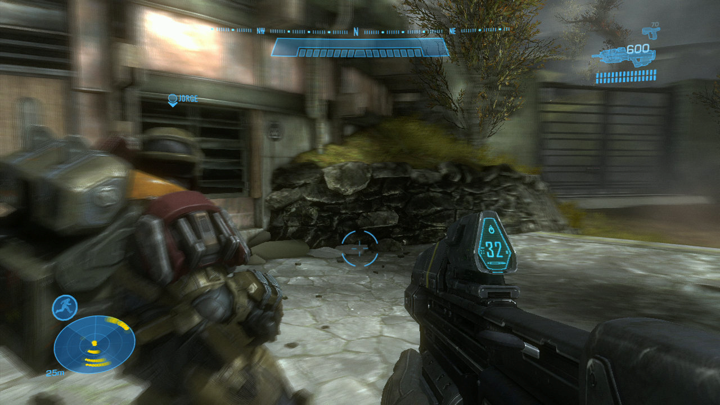
\includegraphics[width=\textwidth]{motion_blur}
		\end{center}
	\end{column}
\end{columns}
\end{frame}

\begin{frame}
	\frametitle{Motion Blur}
	\begin{columns}
		\begin{column}{0.5\textwidth}
			\begin{itemize}
				\item Or we can simply take the results of the last render update and blend them with current render results and blend based on a lerp
			\end{itemize}
		\end{column}
		\begin{column}{0.5\textwidth} 
			\begin{center}
				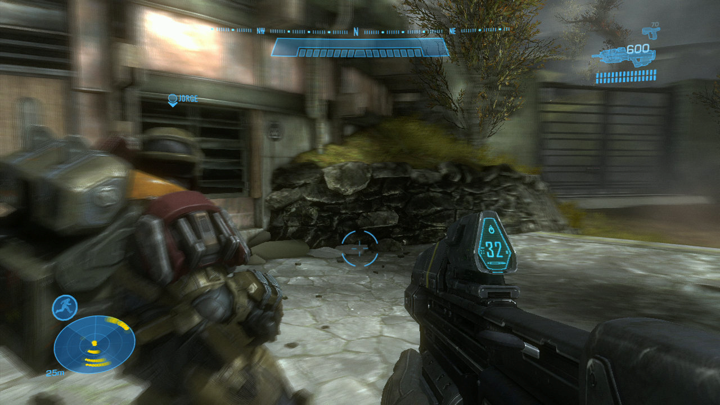
\includegraphics[width=\textwidth]{motion_blur}
			\end{center}
		\end{column}
	\end{columns}
\end{frame}

\begin{frame}
	\frametitle{Depth of Field}
\begin{columns}
	\begin{column}{0.5\textwidth}
		\begin{itemize}
			\item DOF attempts to simulate the effect where object that are too close or too far away appear out of focus
			\item We first have to consider in our scene what range of depth values will be considered in focus. We then need to blur everything that is outside this range
		\end{itemize}
	\end{column}
	\begin{column}{0.5\textwidth} 
		\begin{center}
			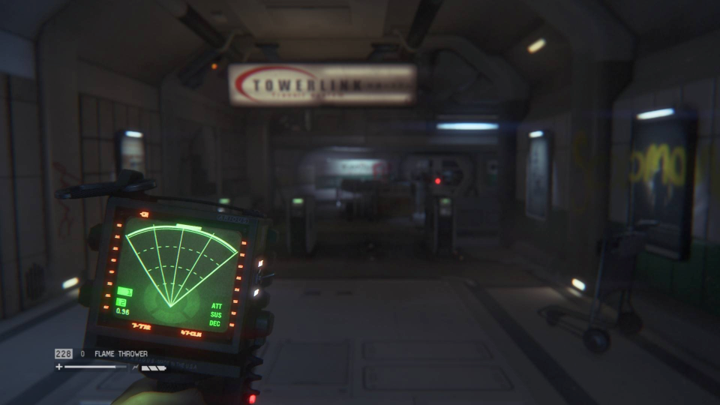
\includegraphics[width=\textwidth]{depth_of_field}
		\end{center}
	\end{column}
\end{columns}	
\end{frame}

\begin{frame}
	\frametitle{Depth of Field}
	\begin{columns}
		\begin{column}{0.5\textwidth}
			\begin{itemize}
				\item Once we have determined this we render a blurred scene to a render texture
			\end{itemize}
		\end{column}
		\begin{column}{0.5\textwidth} 
			\begin{center}
				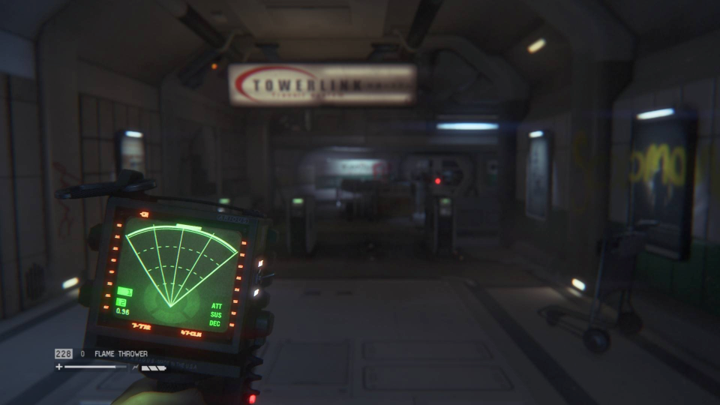
\includegraphics[width=\textwidth]{depth_of_field}
			\end{center}
		\end{column}
	\end{columns}	
\end{frame}

\begin{frame}
	\frametitle{Bloom}
	\begin{columns}
		\begin{column}{0.5\textwidth}
			\begin{itemize}
				\item This attempts to simulate the overloading of the optic nerve if extremely bright areas of a surface are visible
				\item First we render to a smaller render target, usually 1/4 size
			\end{itemize}
		\end{column}
		\begin{column}{0.5\textwidth} 
			\begin{center}
				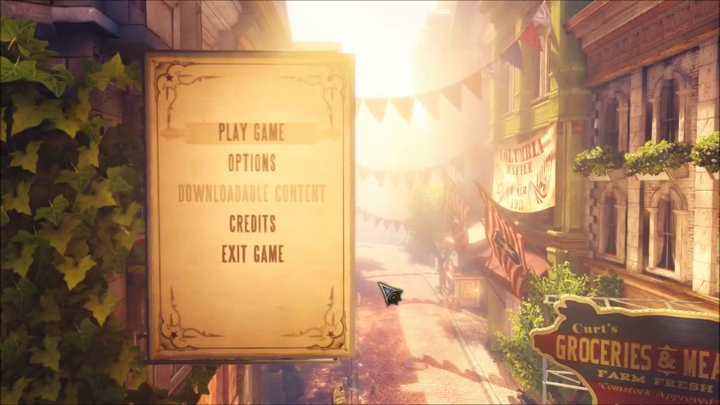
\includegraphics[width=\textwidth]{bloom}
			\end{center}
		\end{column}
	\end{columns}	
\end{frame}

\begin{frame}
	\frametitle{Bloom}
	\begin{columns}
		\begin{column}{0.5\textwidth}
			\begin{itemize}
				\item We then apply a filter (usually Gauss) to this reduced render target, if we apply this filter in multiple passes then we achieve a smoother blur
				\item We then blend the blurred image onto the screen with the original scene 
			\end{itemize}
		\end{column}
		\begin{column}{0.5\textwidth} 
			\begin{center}
				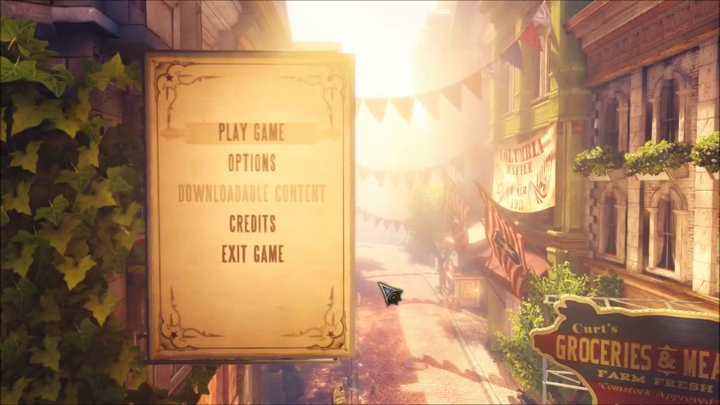
\includegraphics[width=\textwidth]{bloom}
			\end{center}
		\end{column}
	\end{columns}	
\end{frame}

\begin{frame}{Post Processing Stack}
	\begin{itemize}
		\pause\item In theory we can chain post-processing effects together
		\pause\item Essentially we keep rendering to a texturing using different fragment shaders each time
		\pause\item These could be stored in a data structure such as a stack
		\pause\item Once we have completed the last effect on the stack, we then switch to normal rendering and display the result
	\end{itemize}
\end{frame}